%!TeX root = main.tex
%!encoding = UTF-8 Unicode

\section{Demonstration of Noise-Reduction Steps}
First, the influence of the individual noise-reduction steps on high-frequency drain-source-voltage measurements is demonstrated.

\begin{figure}[ht]
	\centering
	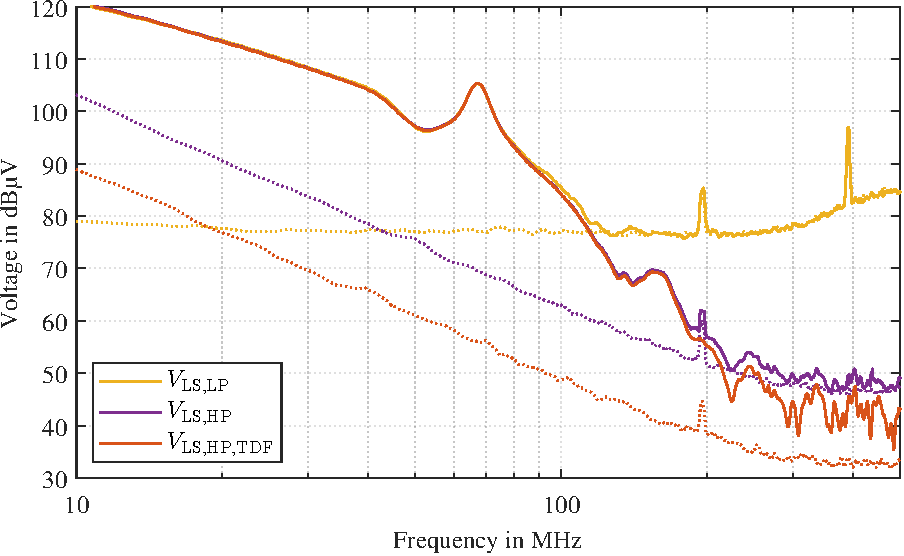
\includegraphics[scale = 1]{figures/7_MeasurementResults/MR_Methodology.pdf}
	\caption{Impact of different noise-reduction steps on the measurement (solid line) and the corresponding noise floor (dotted line).}\label{fig:MR_Methodology}
\end{figure}

Figure~\ref{fig:MR_Methodology} shows the spectrum used later, measured at the active low-side switch of an SiC MOSFET with an active area of \SI{5}{mm^2}, for the low-pass, high-pass, and TDF signals.
For each signal, two measurements are performed: one with DUT operation (signal of interest) and one background measurement without DUT operation to determine the noise floor, which is shown as a dotted line.
To evaluate both quantities in the same spectrum plot, the measured signals are compensated using the transfer functions in \eref{eq:HP_comp} and \eref{eq:TF_Shunt}.



In the low-pass spectrum, which corresponds to conventional measurements, the noise floor is around \SI{76}{dB\micro\volt}, which is sufficient for analyzing the switching transient up to \SI{115}{MHz}.
For higher frequencies, the signal falls below the noise level, which is why the high-pass measurement is necessary.

The high-pass measurement remains above the noise floor up to \SI{220}{MHz}, which is a significant improvement over the low-pass path.
However, the signal still decreases faster over frequency than the noise floor, so the SNR decreases at higher frequencies.
In the high-pass background measurement, the compensated noise floor decreases with frequency because the approximately constant noise measurement is divided by the increasing high-pass gain.

In a final step, the TDF filter is applied in post-processing, further reducing the noise floor by about \SI{15}{dB}.
This enables analysis of the switching transient up to \SI{500}{MHz}.

